\documentclass[11pt,t]{beamer}
\usetheme{Malmoe}
\usepackage[utf8]{inputenc}
\usepackage{amsmath}
\usepackage{amsfonts}
\usepackage{amssymb}
\usepackage[all,cmtip]{xy}
\usepackage{pgfpages}
\usepackage{graphicx}

\pgfpagesuselayout{resize to}[letterpaper,landscape,border shrink=5mm]
\newenvironment{amatrix}[1]{%
  \left[\begin{array}{@{}*{#1}{c}|c@{}}
}{%
  \end{array}\right]
}
\DeclareMathOperator{\rank}{rank}
\DeclareMathOperator{\minor}{minor}
\DeclareMathOperator{\cof}{cof}
\DeclareMathOperator{\adj}{adj}

\newcommand{\R}{\mathbb{R}}
\newcommand{\abs}[1]{\lvert #1\rvert}
%\geometry{landscape,paper=letterpaper}
\beamertemplatenavigationsymbolsempty
\date{}
\author{Math 1410 Linear Algebra}
\title{Determinants}
%\setbeamercovered{transparent} 
%\setbeamertemplate{navigation symbols}{} 
%\logo{} 
%\institute{} 
%\date{} 
%\subject{} 
\begin{document}
\begin{frame}
\titlepage
\end{frame}

%\begin{frame}
%\tableofcontents
%\end{frame}
\section{Calculating Determinants}
\begin{frame}
\frametitle{Introduction}
A \alert{determinant} is a number that can be associated to any $n\times n$ matrix.
\begin{itemize}
\item Definition is \alert{recursive}: first define $2\times 2$ determinants, then $3\times 3$ in terms of $2\times 2$, $4\times 4$ in terms of $3\times 3$, etc.
\item Original use: determining if a system of $n$ equations in $n$ variables has a unique solution.
\item Historically, they pre-date matrices. (By about 2200 years!)
\item Applications include solving systems of equations, volumes in 2, 3 and higher dimensions, differential equations, change of variables in multiple integrals, etc.
\end{itemize}

\end{frame}
\begin{frame}
\frametitle{Determinants: the $2\times 2$ case}

We begin with $2\times 2$ determinants. 
\[
\text{General } 2\times 2 \text{ matrix } A = \begin{bmatrix}a&b\\c&d\end{bmatrix}.
\]
\begin{definition}
The \alert{determinant} of $A=\begin{bmatrix}a&b\\c&d\end{bmatrix}$ is given by
\[
\det A = \begin{vmatrix}
a&b\\c&d
\end{vmatrix} = ad-bc.
\]
\end{definition}
Note: we write either $\det A$ or $\abs{A}$ to denote the determinant of the matrix $A$.
\end{frame}
\begin{frame}
\frametitle{Examples}

\end{frame}
\begin{frame}\frametitle{$2\times 2$ determinants and area}
The \alert{area} of the parallelogram is given by $ad-bc = \begin{vmatrix}
a&b\\c&d
\end{vmatrix}$
\begin{center}
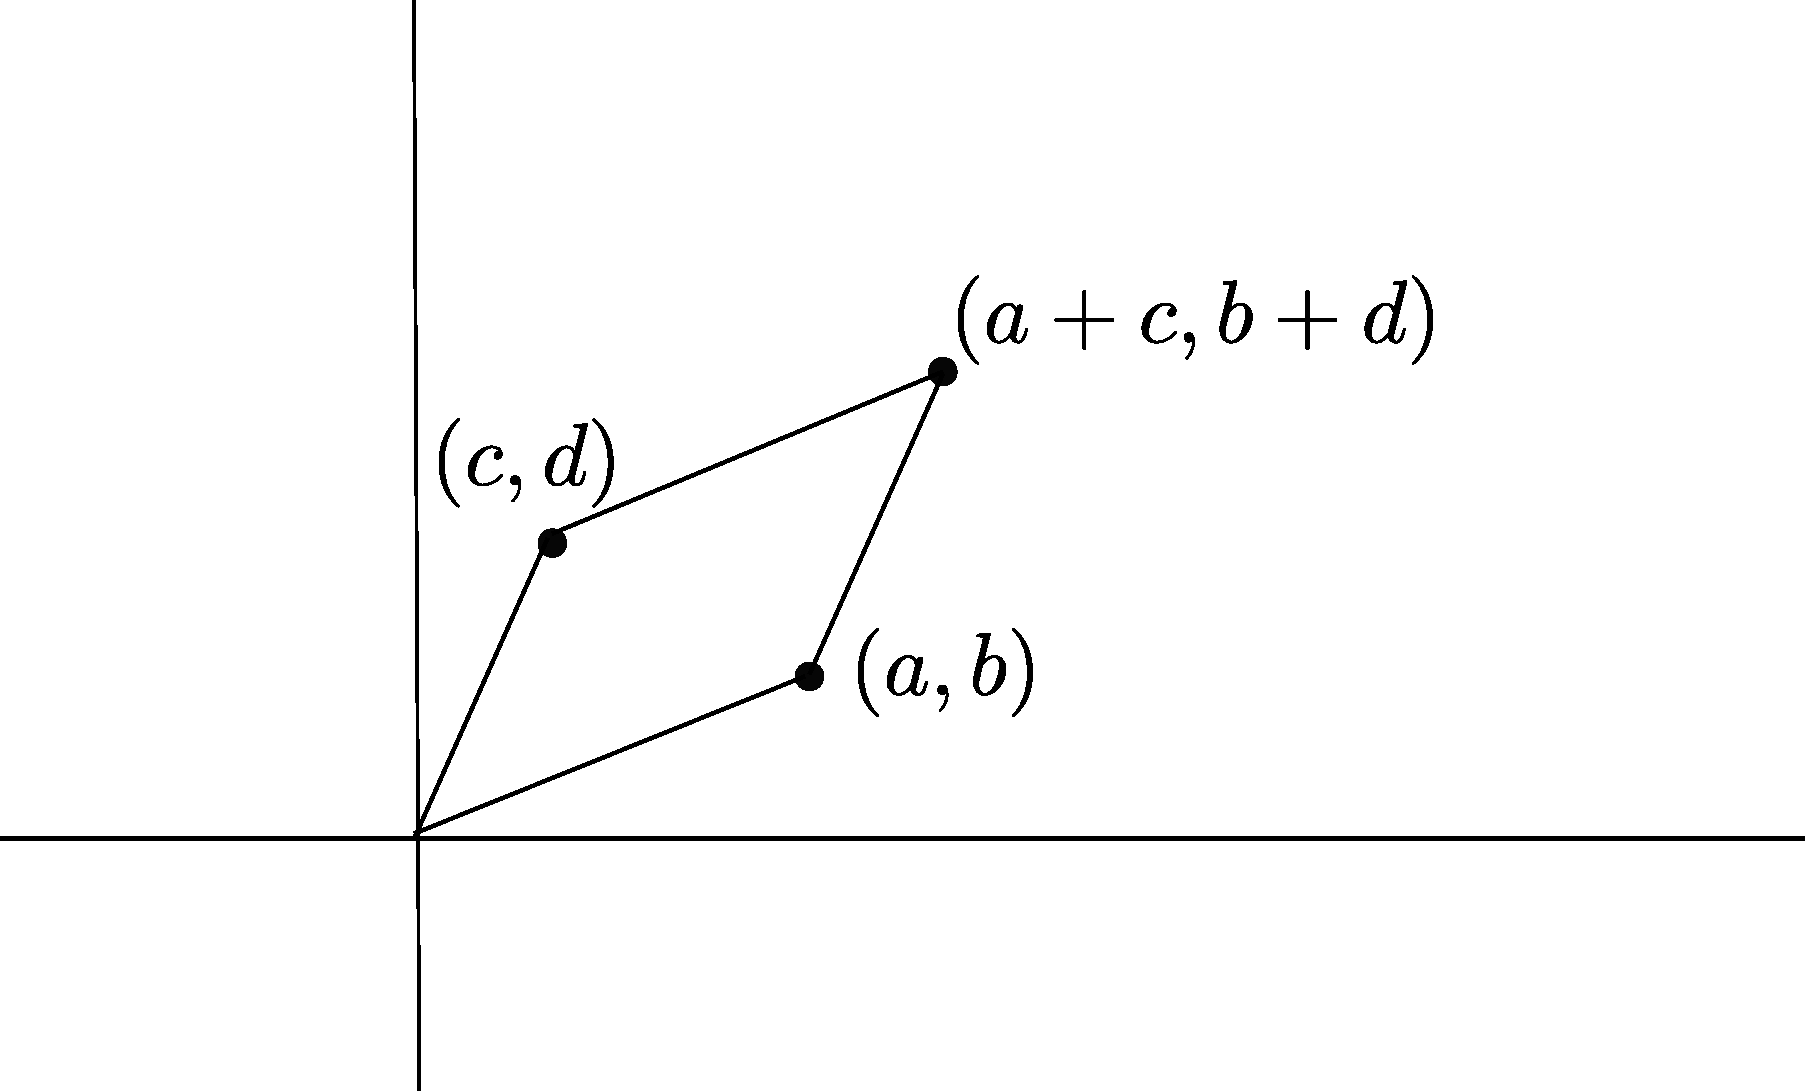
\includegraphics[width=4in]{parallelogram.pdf}
\end{center}
\end{frame}
\begin{frame}
\frametitle{Where does that formula come from?}
Look at the area again:
\begin{center}
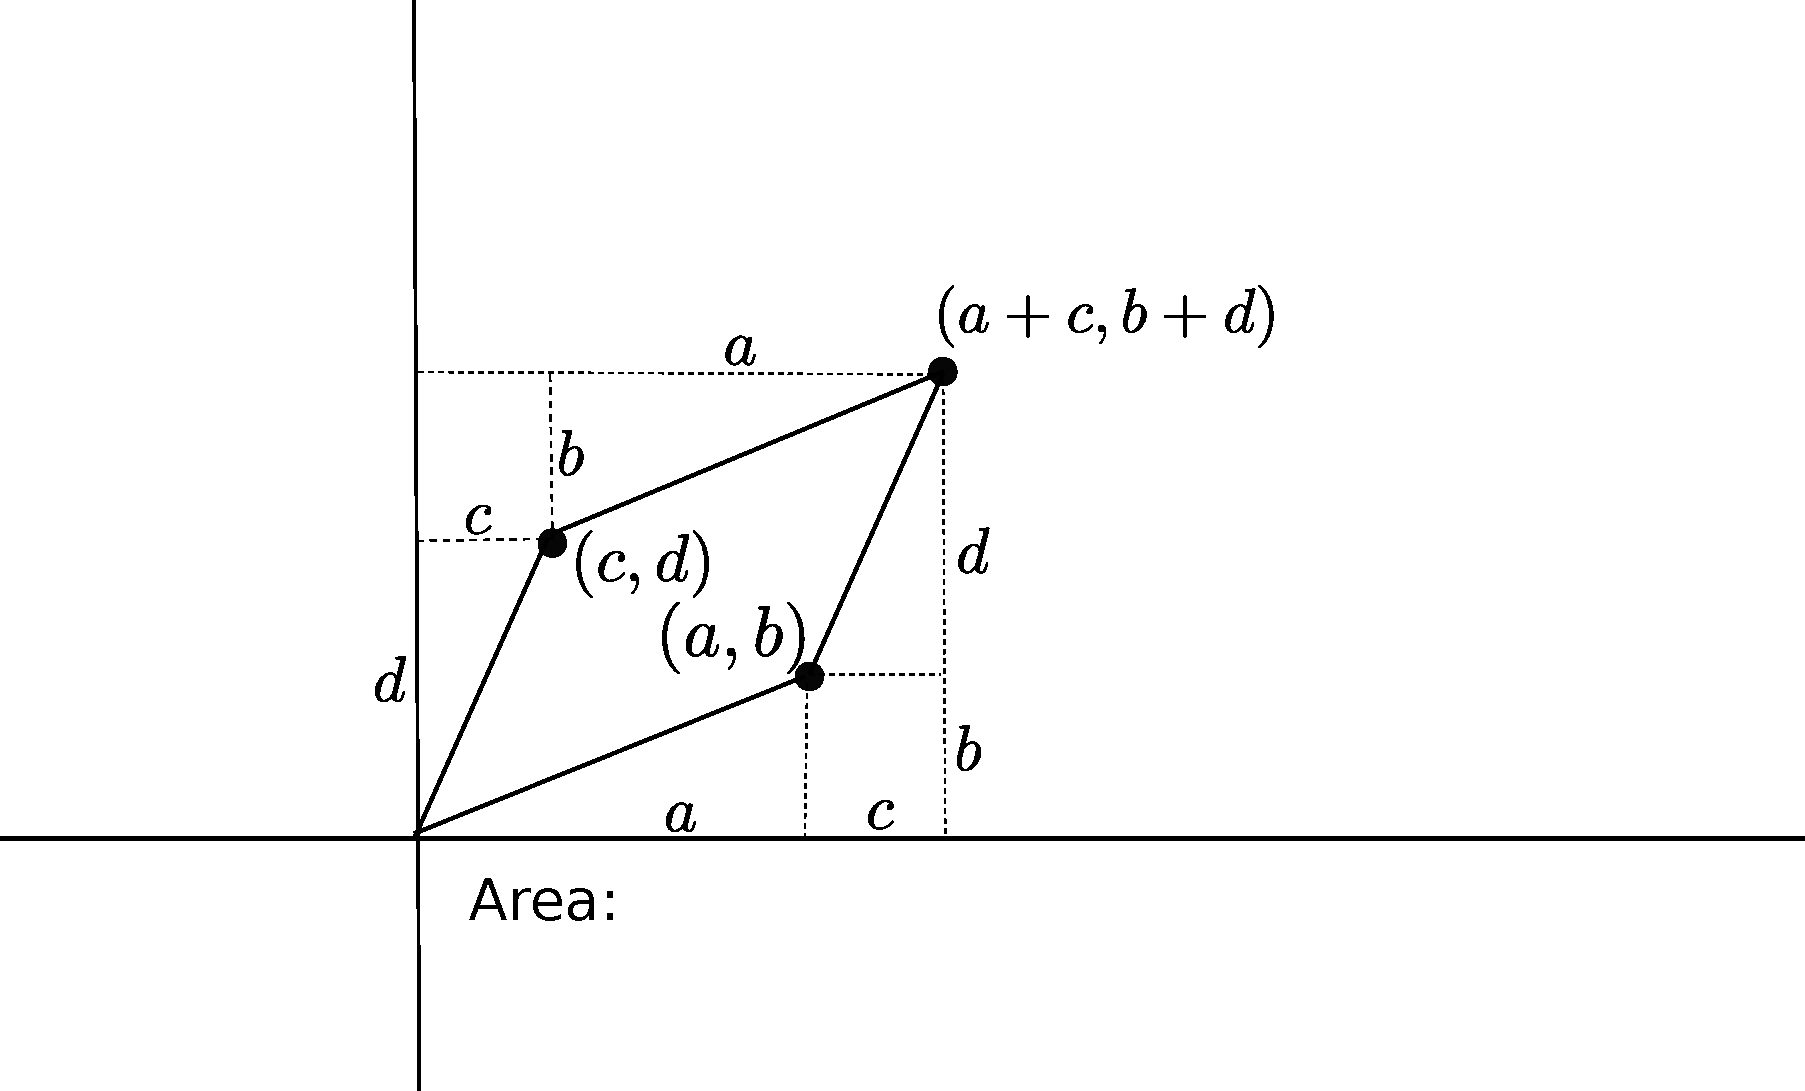
\includegraphics[width=4in]{parallelogram2.pdf}
\end{center}
\end{frame}
\begin{frame}
\frametitle{Minors}
In general, the \alert{$(i,j)$-minor} of an $n\times n$ matrix $A$ is the {\em determinant} of the $(n-1)\times (n-1)$ matrix obtained by deleting row $i$ and column $j$ from $A$. It is denoted by $\minor(A)_{ij}$

\medskip

So, far we only know $2\times 2$ determinants, so let $n=3$. Deleting a row and a column leaves us with a $2\times 2$ matrix, and then we take the determinant. 
\[
\begin{bmatrix}a_{11}&a_{12}&a_{13}\\
    \makebox[0pt][l]{\rule[0.1cm]{0.2\textwidth}{0.7pt}} a_{21}&a_{22}&a_{23}\makebox(-18,0){\rule[1ex]{0.7pt}{3\normalbaselineskip}}\\
a_{31}&a_{32}&a_{33}\end{bmatrix}\to \begin{bmatrix}a_{11}&a_{12}\\a_{31}&a_{32}\end{bmatrix}\to \begin{vmatrix}a_{11}&a_{12}\\a_{31}&a_{32}\end{vmatrix}
\]
Above: computing $\minor(A)_{23}$ for a $3\times 3$ matrix $A$.
\end{frame}
\begin{frame}
\frametitle{Example}

\end{frame}
\begin{frame}
\frametitle{Cofactors}
\begin{definition}
The \alert{$(i,j)$-cofactor} of an $n\times n$ matrix $A$ is denoted by $\cof(A)_{ij}$ and defined by
\[
\cof(A)_{ij} = (-1)^{i+j}\minor(A)_{ij}.
\]
\end{definition}
Note: the only difference between the cofactor and corresponding minor is a sign factor.
\[
(-1)^{i+j} = \begin{cases}+1, & \text{ if } i+j \text{ is even}\\
-1, & \text{ if } i+j \text{ is odd}\end{cases}\]
\[ \Rightarrow \text{  sign pattern: } \begin{bmatrix}+&-&+\\-&+&-\\+&-&+\end{bmatrix}
\]
\end{frame}
\begin{frame}
\frametitle{Example}

\end{frame}
\begin{frame}
\frametitle{The Laplace expansion}
The \alert{Laplace expansion} tells us how to write any $3\times 3$ determinant in terms of $2\times 2$ determinants.
\begin{definition}
Let $A$ be a $3\times 3$ matrix. We define $\det A$ via Laplace expansion along the first row of $A$ as follows:
\begin{align*}
\det A &= a_{11}\cof(A)_{11}+a_{12}\cof(A)_{12}+a_{13}\cof(A)_{13}\\
& = a_{11}\begin{vmatrix}
a_{22}&a_{23}\\a_{32}&a_{33}
\end{vmatrix}-a_{12}\begin{vmatrix}
a_{21}&a_{23}\\a_{31}&a_{33}
\end{vmatrix}+a_{13}\begin{vmatrix}
a_{21}&a_{22}\\a_{31}&a_{32}
\end{vmatrix}
\end{align*}
\end{definition}
\alert{Note:} Expanding along \alert{any row or column} gives the same value for $\det A$.

\bigskip

\alert{Tip:} With the above in mind, pick a row or column with zeros in it!
\end{frame}
\begin{frame}
\frametitle{Example}

\end{frame}
\begin{frame}
\frametitle{Volume}
Just as $2\times 2$ determinants give area, $3\times 3$ determinants give volume:
\begin{center}
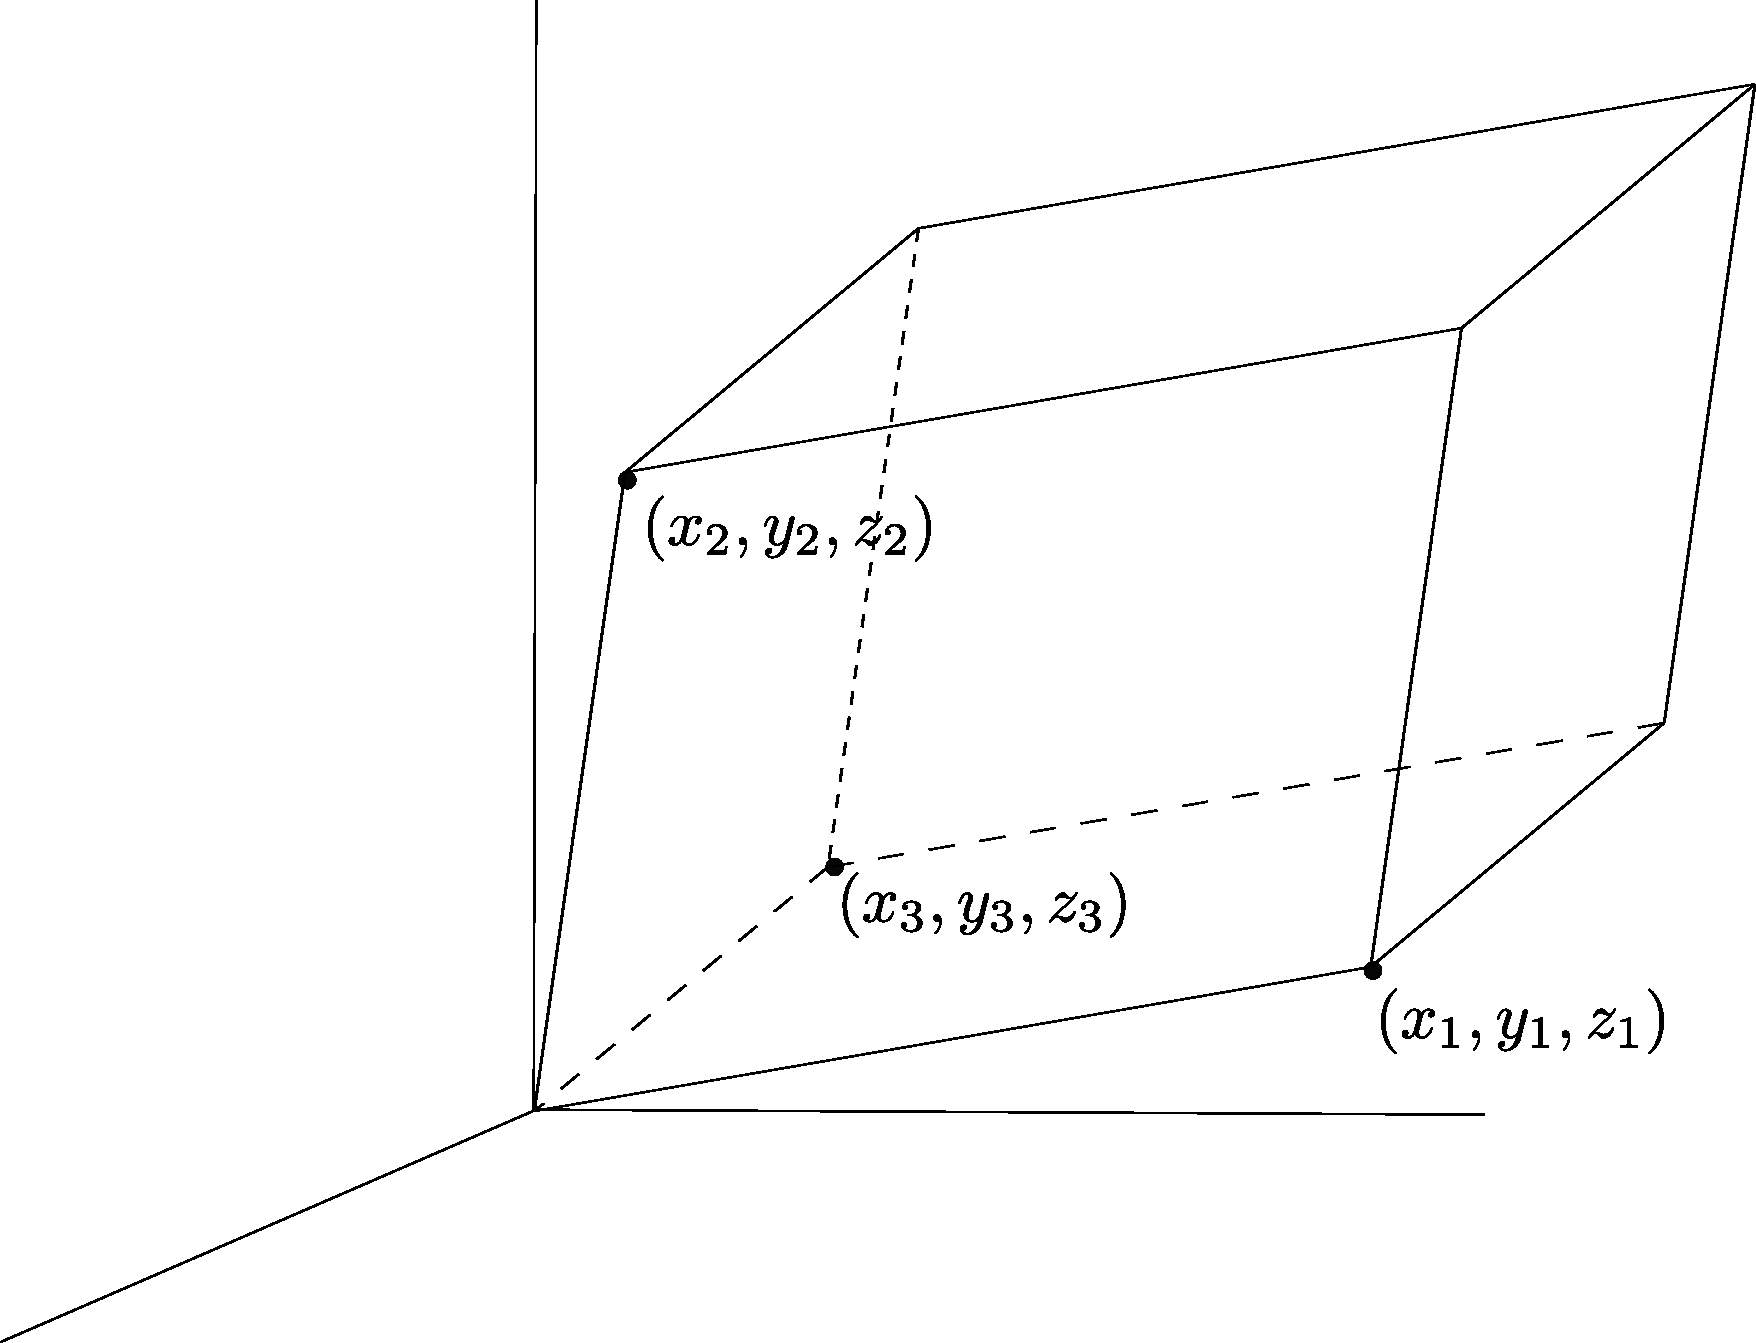
\includegraphics[width=2.5in]{Parallelepiped.pdf}
\end{center}
The volume of the solid shown is $V=\begin{vmatrix}
x_1&y_1&z_1\\x_2&y_2&z_2\\x_3&y_3&z_3
\end{vmatrix}$.

\end{frame}
\begin{frame}
\frametitle{Example}

\end{frame}
\begin{frame}
\frametitle{$4\times 4$ and higher determinants}
Take the same definition: given an $n\times n$ matrix $A$,
\[
\det A = \sum_{i=1}^n a_{1i}\cof(A)_{1i}.
\]
Keep expanding in terms of smaller and smaller determinants until you reach size $2\times 2$.
\end{frame}
\begin{frame}\frametitle{Why the Laplace expansion?}
 One important use of determinants is in deciding whether or not a given matrix is invertible. If $A=\begin{bmatrix}a&b\\c&d\end{bmatrix}$, we row-reduce as follows:
\[
 \begin{bmatrix}a&b\\c&d\end{bmatrix}\xrightarrow[]{R_1\to \frac{1}{a}R_1} \begin{bmatrix}1&b/a\\c&d\end{bmatrix}\xrightarrow[]{R_2\to -cR_1} \begin{bmatrix}1&b/a\\0&\frac{ad-bc}{a}\end{bmatrix}
\]
We know there's an inverse as long as we don't get a row of zeros on the bottom, so we need $ad-bc=\det A\neq 0$

 A similar argument can be applied to a $3\times 3$ matrix $B=\begin{bmatrix}a&b&c\\d&e&f\\g&h&i\end{bmatrix}$, with a bit more work. If you want to see where the $3\times 3$ determinant comes from, try reducing this general matrix to REF and seeing what condition guarantees that there is no row of zeros.
\end{frame}

\begin{frame}
 \frametitle{Triangular matrices}
\begin{itemize}
 \item The \alert{main diagonal} of an $n\times n$ matrix consists of the entries $a_{11},a_{22},\ldots, a_{nn}$.
 \item A matrix $A$ is \alert{upper triangular} if all entries {\em below} the main diagonal (those $a_{ij}$ with $i>j$) are zero.
 \item A matrix $A$ is \alert{lower triangular} if all entries {\em above} the main diagonal (those $a_{ij}$ with $i<j$) are zero.
 \item A matrix $A$ is \alert{triangular} if it is either upper or lower triangular.
\end{itemize}
\begin{theorem}
 If $A$ is an $n\times n$ triangular matrix, then
\[
 \det A = a_{11}a_{22}\cdots a_{nn}.
\]
\end{theorem}
\end{frame}
\begin{frame}\frametitle{Examples}
 
\end{frame}
\begin{frame}\frametitle{Properties of Determinants}
 \begin{theorem}[Effect of row operations]
  Let $A$ be an $n\times n$ matrix. Then:
\begin{enumerate}
 \item If $B$ is obtained from $A$ by exchanging any two rows ($R_i\leftrightarrow R_j$), then $\det B = -\det A$.
 \item If $B$ is obtained from $A$ by multiplying a row by a constant $k$ ($R_i\to kR_i$), then $\det B = k\det A$.
 \item If $B$ is obtained from $A$ by adding a multiple of one row to another ($R_i\to R_i+kR_j$), then $\det B = \det A$.
\end{enumerate}
 \end{theorem}
 \begin{corollary}
\begin{enumerate}
 \item If $A$ has a row of zeros, then  $\det A = 0$.
 \item If one row of $A$ is a multiple of another row, then $\det A = 0$.
\end{enumerate}
 \end{corollary}

\end{frame}
\begin{frame}\frametitle{Examples}
 
\end{frame}
\begin{frame}\frametitle{Proofs}
 We'll look at how these properties work in the $2\times 2$ case. The general argument requires \alert{proof by mathematical induction} (covered in Math 2000).

\end{frame}
\begin{frame}\frametitle{Determinants via row operations}
 Knowing the effect of row operations on determinants means that we can use them to simplify our determinants. Main principles to follow:
\begin{enumerate}
 \item Try to reduce the determinant to triangular form. (Determinants of triangular matrices are easy.)
 \item Try to stick to Type 3 row operations (adding a multiple of one row to another), since \alert{they don't change the value of the determinant}.
 \item If you do use Type 1 or Type 2 row operations, \alert{keep track of the changes}.
\end{enumerate}

\end{frame}
\begin{frame}\frametitle{Example}
 
\end{frame}
\begin{frame}
\frametitle{Scalar Multiplication}
\begin{itemize}
\item Let $A$ be an $n\times n$ matrix.
\item Let $B$ be obtained from $A$ by multiplying row $i$ of $A$ by a nonzero scalar $k$.
\item We know that $\det B = k\det A$.
\item What can we conclude about $\det (kA)$? 
\end{itemize}
(Recall that $kA$ is formed by multiplying \alert{all} rows of $A$ by $k$.)
\end{frame}
\begin{frame}
\frametitle{Determinants of Elementary Matrices}
What are the determinants of the three types of elementary matrix? Recall that:
\begin{enumerate}
\item $\det I_n = 1$.
\item An elementary matrix $E$ is obtained from $I_n$ via a \alert{single} row operation.
\end{enumerate}
\end{frame}
\begin{frame}
\frametitle{Determinant of a product}
\begin{theorem}
Let $A$ and $B$ be any $n\times n$ matrices. Then
\[
\det (AB) = \det A \det B.
\]
\end{theorem}
\begin{example}
Consider $A = \begin{bmatrix}2&-1\\3&5\end{bmatrix},\, B = \begin{bmatrix}-3&4\\7&-2\end{bmatrix}$.


\end{example}
\end{frame}
\begin{frame}
\frametitle{Proof that $\det (AB)=\det A\det B$}
Two cases:
\begin{enumerate}
\item $A$ is not invertible, so $A=E_k\cdots E_2E_1R$, where $R$ (REF) has a row of zeros.\\
 Therefore $RB$ has a row of zeros, so $\det (RB)=0$. \\
 Now note $\det A$, $\det (AB)$ are obtained from $\det R$, $\det (RB)$ by elementary row operations, so $\det A=0$ and $\det (AB) = 0$.
\item $A$ is invertible, so $A=E_k\cdots E_2E_1$ is a product of elementary matrices.\\
Note $A$ obtained from $I_n$ via elementary row operations.\\
Also $AB$ obtained from $B$ via the \alert{same} row operations.
\end{enumerate}
\end{frame}
\begin{frame}
\frametitle{Determinant of an invertible matrix}
\begin{theorem}
Let $A$ be an $n\times n$ matrix. Then $A$ is invertible if and only if $\det A\neq 0$, and if $A$ is invertible, then $\det A^{-1} = \dfrac{1}{\det A}$.
\end{theorem}
\begin{proof}
\vspace{1.7in}
\end{proof}
\end{frame}
\begin{frame}
\frametitle{Example}

\end{frame}
\begin{frame}
\frametitle{Determinants and transpose}
\begin{theorem}
For any $n\times n$ matrix $A$, $\det A = \det A^T$.
\end{theorem}
\alert{Consequence}: we can also simplify a determinant using column operations. (Why?)
\end{frame}
\begin{frame}
\frametitle{Example}

\end{frame}
\begin{frame}
\frametitle{Example}

\end{frame}
\section{Applications of Determinants}
\begin{frame}
\frametitle{The adjugate matrix}
\alert{Recall}: For any $n\times n$ matrix $A$, the $(i,j)$-cofactor of $A$ is given by
\[
\cof(A)_{ij} = (-1)^{i+j}\operatorname{minor}(A)_{ij}.
\]
If we replace every entry $a_{ij}$ in $A$ by the corresponding cofactor, we obtain the \alert{cofactor matrix} of $A$:
\[
\cof(A) = [\cof(A)_{ij}]_{n\times n}.
\]
The \alert{adjugate} of $A$ is the {\em transpose} of the cofactor matrix:
\[
\adj(A) = \cof(A)^T.
\]
(The adjugate is sometimes referred to as the {\em adjoint} of $A$, but this has another meaning.)
\end{frame}
\begin{frame}
\frametitle{Example}

\end{frame}
\begin{frame}
\frametitle{A determinant formula for $A^{-1}$}
\begin{theorem}
Let $A$ be an $n\times n$ matrix such that $\det A\neq 0$. Then $A$ is invertible, and
\[
A^{-1} = \frac{1}{\det A}\adj(A).
\]
\end{theorem}
\alert{Remark}: For a $2\times 2$ matrix $A=\begin{bmatrix}a&b\\c&d\end{bmatrix}$, this theorem provides a formula some of you may have seen:
\[
A^{-1} = \frac{1}{ad-bc}\begin{bmatrix}d&-b\\-c&a\end{bmatrix}.
\]

\end{frame}
\begin{frame}
\frametitle{Example}

\end{frame}
\begin{frame}
\frametitle{Sketch of the proof}
Let $A$ be an $n\times n$ matrix with $\det A\neq 0$. It suffices to show that
\[
A\adj(A) = \begin{bmatrix}
a_{11}&\cdots & a_{1n}\\
a_{21}&\cdots & a_{2n}\\
\vdots &\ddots &\vdots\\
a_{n1}&\cdots &a_{nn}
\end{bmatrix}
\begin{bmatrix}
\cof(A)_{11}&\cdots &\cof(A)_{n1}\\
\cof(A)_{12}&\cdots &\cof(A)_{n2}\\
\vdots &\ddots &\vdots\\
\cof{A}_{1n}&\cdots & \cof(A)_{nn}
\end{bmatrix} = \det(A)I_n
\]
\end{frame}
\begin{frame}
\frametitle{When to use the determinant formula}
Take any $4\times 4$ matrix of integers, and compare finding $A^{-1}$ using row operations to the determinant formula. The old method is \alert{much less work}.

Why use the new formula? There are a couple of cases where it works better:
\begin{enumerate}
\item Matrices with non-integer entries. (Especially decimals or irrational numbers.) This is generally done with a calculator or computer.
\item Matrices with entries that are \alert{functions}.
\end{enumerate}

\end{frame}
\begin{frame}
\frametitle{Example}
The \alert{spherical coordinate} transformation for calculus in three variables is given by $T(\rho, \theta, \phi) = (x,y,z)$, where
\begin{align*}
x & = \rho\cos\theta\sin\phi\\
y & = \rho\sin\theta\sin\phi\\
z & = \rho\cos\phi
\end{align*}
The \alert{derivative} of this transformation is given by
\[
DT = \begin{bmatrix}
\frac{\partial x}{\partial \rho} & \frac{\partial x}{\partial \theta} & \frac{\partial x}{\partial \phi}\\
\frac{\partial y}{\partial \rho} & \frac{\partial y}{\partial \theta} & \frac{\partial y}{\partial \phi}\\
\frac{\partial z}{\partial \rho} & \frac{\partial z}{\partial \theta} & \frac{\partial z}{\partial \phi}
\end{bmatrix} = 
\begin{bmatrix}
\cos\theta\sin\phi & -\rho\sin\theta\sin\phi & \rho\cos\theta\cos\phi\\
\sin\theta\sin\phi & \rho\cos\theta\sin\phi & \rho\sin\theta\cos\phi\\
\cos\phi & 0 &-\rho\sin\phi 
\end{bmatrix}
\]
For what values of $\rho, \theta$, and $\phi$ is the derivative matrix invertible?
\end{frame}
\begin{frame}
\frametitle{Cramer's Rule}

\alert{Cramer's Rule} applies to systems of $n$ equations in $n$ variables of the form
\[
AX=\begin{bmatrix}
a_{11}&\cdots&a_{1n}\\
\vdots&\ddots&\vdots\\
a_{n1}&\cdots&a_{nn}
\end{bmatrix}\begin{bmatrix}x_1\\\vdots\\x_n\end{bmatrix} = \begin{bmatrix}b_1\\\vdots\\b_n\end{bmatrix}=B,
\]
where $A$ is \alert{invertible}. We have
\[
X = A^{-1}B = \frac{1}{\det A}\adj(A)B,
\]
which means $x_j$ is given by $\dfrac{1}{\det A}(\text{row } j \text{ of } \adj(A))B$. \\

\end{frame}
\begin{frame}
\frametitle{Cramer's Rule, again}
Given a system $AX=B$ of $n$ equations in $n$ variables \alert{with $A$ invertible}, let $A_i$ be the matrix obtained by replacing column $i$ of $A$ by $B$. Then for each $i=1,\ldots, n$,
\[
x_i = \frac{\det A_i}{\det A}.
\]

\bigskip

\alert{Caution}: Once again, this result isn't really useful for systems with integer coefficients. (Compared to our previous method.) Its main use is when the coefficients are non-integers or functions.
\end{frame}
\begin{frame}
\frametitle{Example}

\end{frame}
\end{document}